\documentclass[a4paper]{article}
\usepackage{amsmath, amssymb, amsfonts}
\usepackage[margin=1in]{geometry}
\usepackage{graphicx}
\usepackage{tikz}
\usepackage{esint}
\usepackage{mathtools}
\setlength{\parindent}{0em}
\setlength{\parskip}{1ex}
\newcommand{\vct}[1]{\overrightarrow{#1}}
\newcommand{\dif}{\mathrm{d}}
\newcommand{\pd}[2]{\frac{\partial {#1}}{\partial {#2}}}
\newcommand{\dd}[2]{\frac{\mathrm{d} {#1}}{\mathrm{d} {#2}}}
\newcommand{\C}{\mathbb{C}}
\newcommand{\R}{\mathbb{R}}
\newcommand{\Q}{\mathbb{Q}}
\newcommand{\Z}{\mathbb{Z}}
\newcommand{\N}{\mathbb{N}}
\newcommand{\fn}[3]{{#1}\colon {#2} \rightarrow {#3}}
\newcommand{\avg}[1]{\langle {#1} \rangle}
\newcommand{\Sum}[2][0]{\sum_{{#2} = {#1}}^{\infty}}
\newcommand{\Lim}[1]{\lim_{{#1} \rightarrow \infty}}
\newcommand{\Binom}[2]{\begin{pmatrix} {#1} \cr {#2} \end{pmatrix}}
\newcommand{\duline}[1]{\underline{\underline{#1}}}

\begin{document}
\paragraph{Osnovni delci.} V 30. letih so bili znani delci \(p\), \(n\), \(e^\pm\) in \(\nu_e\) - na kratko; delci, ki jih je bilo mogoče pridobiti z jedrskimi reakcijami.
V obliki kozmičnih žarkov so nato odkrili mione (\(m = 104\,\mathrm{MeV}\)) in pione (\(m = 140\,\mathrm{MeV}\)), za katere sta značilni sledeči reakciji:
\[\mu^\pm \to e^\pm + X\]
\[\pi^\pm \to \mu^\pm + X\]
Mioni torej nastanejo iz pionov, ti pa nastanejo pri sledečih reakcijah:
\[p + p \to p + p + \pi^- + \pi^+\]
\[p + p \to p + n + \pi^+\]
\[p + p \to p + p + \pi^0\]
Na podlagi teh reakcij moremo sklepati sledeče:
\begin{enumerate}
    \item Vsota števila protonov in nevtronov je konstantna.
    \item Število pionov se ne ohranja.
    \item Naboj se ohranja.
\end{enumerate}
\paragraph{Pospeševalnik.} \text{} \\
\begin{figure}[h!]
    \centering
    \begin{tikzpicture}
        \node (p) at (-4, 0) {\(p\)};
        \draw[->] (-3.75, 0) -- (-1.25, 0);
        \draw (-1, -0.5) rectangle (0, 0.5);
        \node (1) at (-0.5, -0.75) {Tarča 1};
        \draw (0, 1.5) circle (0.25);
        \filldraw (0, 1.5) circle (0.03);
        \node (B) at (-0.5, 1.5) {\(\vct{B}\)};
        \draw[->] (0.25, 0) arc (90:0:2);
        \draw[->] (0.25, 0) arc (270:360:2);
        \node (minus) at (2.75, 1.8) {\(\pi^-\)};
        \node (plus) at (2.75, -1.8) {\(\pi^+\)};
        \draw (1.75, -3.25) rectangle (2.75, -2.25);
        \node (2) at (2.25, -3.5) {Tarča 2};
    \end{tikzpicture}
\end{figure} \\
Na podlagi radija krožnice, po kateri potuje \(\pi^+\),
lahko izračunamo gibalno količino pionov, kar nam pove minimalno energijo delca, ki je priletel v tarčo.
Sipalni presek v odvisnosti od mase delca, ki prileti v tarčo:
\[\sigma = \frac{\sigma_0}{(E-E_R)^2 + \frac{\Gamma^2}{2}}\]
Tu je \(\Gamma\) širina krivulje okoli \(E_R\) pri polovici maksimalne vrednosti \(\sigma\). Funkcija je podobna funkciji za resonanco, in v resnici za nekakšno resonanco tudi gre. \\
Reakciji
\[\pi^- p \to \pi^- p\]
\[\pi^- p \to \pi^0 n\]
imata enako resonanco (označimo \(\Delta^0\)) in posledično enak sipalni presek.
Imamo še tri druge vrste resonance, in sicer \(\Delta^+\), \(\Delta^-\) in \(\Delta^{++}\) - za reakcijo \(\pi^+ p \to \pi^+ p\).
Pri vrstah resonance gre v bistvu za to, koliko naboja je vključenega. Različne reakcije z enako resonanco imajo enako energijo \(E_R\) in širino \(\Gamma\).
\paragraph{Izospin.} Protoni in nevtroni imajo spin \(\displaystyle{\frac{1}{2}}\) z možnima projekcijama \(\displaystyle{m = \pm \frac{1}{2}}\); \\[2mm] pioni imajo spin \(1\) s projakcijami
\(m = 0, \pm 1\); \\[2mm] za resonance \(\Delta^-, \Delta^0, \Delta^+, \Delta^{++}\) pa definiramo skupni spin \(s = \frac{3}{2}\) s projekcijami \(m = \displaystyle{\pm \frac{1}{2}, \pm \frac{3}{2}}\). \\[2mm]
Definiramo izospin \(I\):
\[|p\rangle = |I = \frac{1}{2}, I_3 = \frac{1}{2}\rangle\]
\[|n\rangle = |I = \frac{1}{2}, I_3 = -\frac{1}{2}\rangle\]
\[|\pi^+\rangle = |I = 1, I_3 = 1\rangle\]
\[|\Delta^+\rangle = |I = \frac{3}{2}, I_3 = \frac{1}{2}\rangle\]
\[|\Delta^{++}\rangle = |I = \frac{3}{2}, I_3 = \frac{3}{2}\rangle\]
To nam omogoči, da razmerja med sipalnimi preseki določamo na podlagi izospina.
\paragraph{Čudni delci.} Za primer vzemimo nastanek kaonov \(K\):
\[p + p \to p + p + K^+ + K^-\]
Ta reakcija poteče. Reakcija
\[p + p \to p + n + K^+\]
pa ne poteče. Delci \(K\) nastajajo samo v parih. Razpad kaonov pa poteka takole:
\[K^+ \to \mu^+\nu_m\]
Uvedemo kvantno število \(S\), ki pomeni čudnost delca. V primeru kaonov velja
\[S(K^+) = +1\]
\[S(K^-) = -1\]
\[S(K^0) = +1\]
\[S(\overline{K^0}) = -1\]
Čudnost se pri nastanku kaonov ohranja pri razpadu pa ne. Splošneje se čudnost ohranja pri močni interakciji, pri šibki pa ne. \\[3mm]
Zaenkrat obravnavane delce razdelimo na skupine na podlagi tega, iz koliko kvarkov so sestavljeni. Delce, ki niso sestavljeni iz kvarkov, imenujemo leptoni:
\(e, \mu, \nu_e, \nu_\mu\). Delce, ki so sestavljeni iz kvarkov, imenujemo hadroni, in jih delimo na dve skupine. Barioni (\(p, n, \Delta\)) so sestavljeni
iz treh kvarkov, mezoni (\(\pi, K\)) pa iz dveh. Število barionov se v reakcijah ohranja, število mezonov pa ne.
\newpage
\paragraph{Mezoni.} Vseh mezonov skupaj je osem: \\
\(\pi:~I=1,~I_3=-1, 0, 1,~S=0\) \\
\(K:~I=\frac{1}{2},~I_3= -\frac{1}{2},\,\frac{1}{2},~S=-1, 1\) \\
\(\eta:~I = 0,~S = 0\)
\begin{figure}[h!]
    \centering
    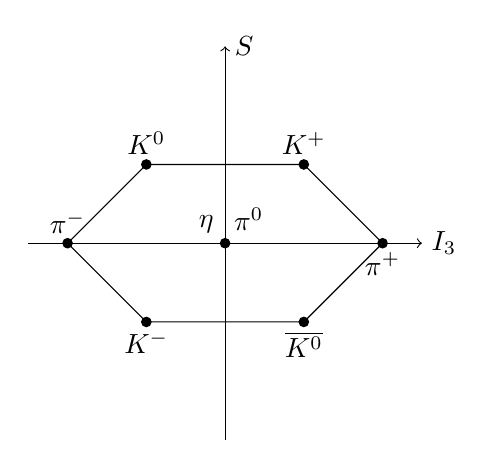
\begin{tikzpicture}[scale=2]
        \draw[->] (-1.25, 0) -- (1.25, 0) node[right] {\(I_3\)};
        \draw[->] (0, -1.25) -- (0, 1.25) node[right] {\(S\)};

        \draw (0.5, 0.5) -- (1, 0) -- (0.5, -0.5) -- (-0.5, -0.5) -- (-1, 0) -- (-0.5, 0.5) -- (0.5, 0.5);
        \filldraw (0.5, 0.5) circle (0.03) node[above] {\(K^+\)};
        \filldraw (0.5, -0.5) circle (0.03) node[below] {\(\overline{K^0}\)};
        \filldraw (-0.5, -0.5) circle (0.03) node[below] {\(K^-\)};
        \filldraw (-0.5, 0.5) circle (0.03) node[above] {\(K^0\)};
        \filldraw (1, 0) circle (0.03) node[below] {\(\pi^+\)};
        \filldraw (-1, 0) circle (0.03) node[above] {\(\pi^-\)};
        \filldraw (0, 0) circle (0.03);
        \node (p) at (-0.12, 0.12) {\(\eta\)};
        \node (p) at (0.15, 0.15) {\(\pi^0\)};
    \end{tikzpicture}
\end{figure} \\
Njihova skupna lastnost je \(J=0\).
\paragraph{Barioni.} Tudi teh je osem (resonance \(\Delta\) ne štejejo), druži pa jih lastnost \(J = \frac{1}{2}\). \\
\begin{figure}[h!]
    \centering
    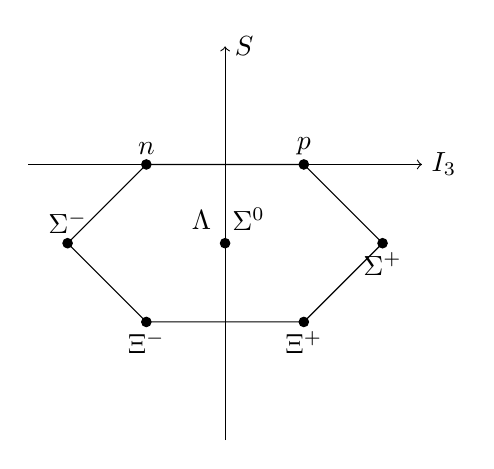
\begin{tikzpicture}[scale=2]
        \draw[->] (-1.25, 0.5) -- (1.25, 0.5) node[right] {\(I_3\)};
        \draw[->] (0, -1.25) -- (0, 1.25) node[right] {\(S\)};

        \draw (0.5, 0.5) -- (1, 0) -- (0.5, -0.5) -- (-0.5, -0.5) -- (-1, 0) -- (-0.5, 0.5) -- (0.5, 0.5);
        \filldraw (0.5, 0.5) circle (0.03) node[above] {\(p\)};
        \filldraw (0.5, -0.5) circle (0.03) node[below] {\(\Xi^+\)};
        \filldraw (-0.5, -0.5) circle (0.03) node[below] {\(\Xi^-\)};
        \filldraw (-0.5, 0.5) circle (0.03) node[above] {\(n\)};
        \filldraw (1, 0) circle (0.03) node[below] {\(\Sigma^+\)};
        \filldraw (-1, 0) circle (0.03) node[above] {\(\Sigma^-\)};
        \filldraw (0, 0) circle (0.03);
        \node (p) at (-0.15, 0.15) {\(\Lambda\)};
        \node (p) at (0.15, 0.15) {\(\Sigma^0\)};
    \end{tikzpicture}
\end{figure}
Nekaj teh delcev so odkrili preko delca \(\Omega^{-}\):
\[K^-p \to \Omega^-K^0K^+\]
\[\Omega^- \to \Xi^0 \pi^-\]
\[\Xi^0 \to \Lambda^0 \pi^0\]
\[\Lambda^0 \to p\pi^-\]
Mimogrede omenimo, da ima \(\Omega^-\) čudnost \(S = -3\). (Najbolj povprečen delec v zgodovini delcev.)
\paragraph{Kvarki.} Kot smo že omenili, so barioni sestavljeni iz treh kvarkov, mezoni pa iz treh.
Zaenkrat so za nas relevantni kvarki \(u\), \(d\) in \(s\) ter njihovi antikvarki.
\begin{table}[h!]
    \centering
    \begin{tabular}{c c}
        \begin{tabular}{c|c c c}
            & \(e\) & \(S\) & \(I_3\) \\
            \hline
            \(u\) & \(2/3\,e_0\) & 0 & \(1/2\) \\
            \(d\) & \(-1/3\,e_0\) & 0 & \(-1/2\) \\
            \(s\) & \(-1/3\,e_0\) & -1 & \(0\) \\
        \end{tabular} \hspace{1cm} & \hspace{1cm}
        \begin{tabular}{c|c c c}
            & \(e\) & \(S\) & \(I_3\) \\
            \hline
            \(\overline{u}\) & \(-2/3\,e_0\) & 0 & \(-1/2\) \\
            \(\overline{d}\) & \(1/3\,e_0\) & 0 & \(1/2\) \\
            \(\overline{s}\) & \(1/3\,e_0\) & 1 & \(0\) \\
        \end{tabular}
    \end{tabular}
\end{table} \\
Posamezni vrsti kvarka rečemo okus (tako imata npr. kvarka \(u\) in \(\overline{u}\)) naprotno enak okus.
Tako je na primer \(p = uud\), \(n = udd\), \(\pi = u\overline{d}\). Vrednosti \(e\), \(S\) in \(I_3\) pa samo seštejemo.
\paragraph{Mezoni.} Različne kombinacije \(q\overline{q}\) nam dajo \(3\cdot3=9\) različnih možnih mezonov. Narišimo še enkrat diagram \(S(I_3)\) \\[1mm]
\begin{figure}[h!]
    \centering
    \begin{tikzpicture}[scale=2]
        \draw[->] (-1.25, 0) -- (1.25, 0) node[right] {\(I_3\)};
        \draw[->] (0, -1.25) -- (0, 1.25) node[right] {\(S\)};

        \filldraw (0.5, 0.5) circle (0.03) node[above] {\(u\overline{s} = K^+\)};
        \filldraw (0.5, -0.5) circle (0.03) node[below] {\(s\overline{d} = \overline{K^0}\)};
        \filldraw (-0.5, -0.5) circle (0.03) node[below] {\(s\overline{u} = K^-\)};
        \filldraw (-0.5, 0.5) circle (0.03) node[above] {\(d\overline{s}K^0\)};
        \filldraw (1, 0) circle (0.03) node[below] {\(u\overline{d}\)};
        \filldraw (-1, 0) circle (0.03) node[above] {\(d\overline{u}\)};
        \filldraw (0, 0) circle (0.03);
    \end{tikzpicture}
\end{figure} \\
Vsredini se nahajajo kombinacije \(u\overline{u}\), \(d\overline{d}\) in \(s\overline{s}\) ter linearne kombinacije teh treh stanj.
Označimo \[|\eta'\rangle = |u\overline{u} + d\overline{d} + s\overline{s}\rangle\]
Skupaj imamo torej devet stanj.
\paragraph{Prehodi med stanji.} Med vsemi stanji v tabeli lahko prehajamo z menjavami kvarkov. Na primer:
\[K^0 \xrightarrow{d \to u} K^+\]
\[\pi^- \xrightarrow{d \to s} K^-\]
Kar pa se tiče stanje \(\eta'\), označimo: \\
\(|u\overline{u}\rangle = |1\rangle\) \\
\(|d\overline{d}\rangle = |2\rangle\) \\
\(|u\overline{s}\rangle = |3\rangle\) \\
Tedaj je \[\eta' = \frac{1}{\sqrt{3}}\left(|1\rangle + |2\rangle + |3\rangle\right)\]
ortonormirano stanje. Imamo še dve drugi stanji, ki sta nanj pravokotni:
\[|\pi^0\rangle = \frac{1}{\sqrt{2}}\left(|1\rangle - |2\rangle\right)\]
\[|\eta\rangle = \frac{1}{\sqrt{6}}\left(|1\rangle + |2\rangle - 2|3\rangle\right)\]
Koeficienti so nastavljeni tako, da so stanja ortonormirana.
\paragraph{Spin mezonov.} Valovna funkcija delcev, sestavljenih iz dveh kvarkov:
$$\psi = \psi_{\text{okus}} \psi_{\text{spin}} \psi (\vct{r})$$
$\psi_{\text{okus}}$ dobimo kot vsoto stanj $|u \overline{u}\,\rangle$, $|d\overline{d}\,\rangle$ in podobno
- še vedno uporabljamo samo kvarke $u$, $d$ in $s$ ter pripadajoče antikvarke. \\
Za spin imamo več močnosti:
$$|\downarrow \downarrow\,\rangle,~~|\downarrow \uparrow\,\rangle,~~|\uparrow \downarrow\,\rangle,~~|\uparrow \uparrow\,\rangle$$
Možnost $|\uparrow \uparrow\,\rangle$ predstavimo kot $|1, 1\rangle$, možnost $|\downarrow, \downarrow\,\rangle$ predstavimo kot $|1, -1\rangle$.
Preostali dve možnosti nam data $|1, 0\rangle$, bolj specifično velja
$$|1, 0\rangle = \frac{1}{\sqrt{2}}\,\left(|\uparrow\downarrow\,\rangle + |\downarrow\uparrow\,\rangle\right)$$
\paragraph{Globoko neelastično sipanje.} Na ta način želimo dokazati, da so kvarki delci. Hitro se je pokazalo, da
so vedno vezani (kajti prostih kvarkov ni bilo mogoče najti). Drugi poskus je bil s sipanjem elektronov na protonih.
Lahko pa dosežemo proces $e^- p ^+ \to e^- X$, kjer je $X$ nek delec. To pomeni, da se je elektron sipal na
točkastih sestavnih delih protona, ki so se nato prerazporedili v nek drug delec.
\paragraph{Odkritje kvarka $c$} Leta 1974 so odkrili nov delec $J$ (ali delec $\psi$ - eksperiment so izvedli v dveh laboratorijih hkrati).
Ustvarili so tako, da so pri velikih kinetičnih energijah med sabo trčili dva elektrona, rezultat česar je gotovo mezon, saj se število barionov ohranja (na nič).
Novi delec je imel maso $3.1\,\mathrm{GeV/c^2}$, sestavljen je iz $c\overline{c}$. Kvark $c$ ima naboj $\displaystyle{\frac{2}{3}e_0}$ in maso $\sim 1.5\,\mathrm{GeV}$.
Tvori tudi kombinacije z ostalimi kvarki:
\begin{align*}
    D^+ & = c\overline{d} & D^- & = \overline{c}d \\
    D^0 & = c\overline{u} & \overline{D^0} & = \overline{c}u \\
    D_s^+ & = c\overline{s} & D_s^- & = \overline{c}s \\
\end{align*}
\paragraph{Odkritje kvarka $b$} Leta 1977 so odkrili delec $Y$, sestavljen iz delcev $B^0\overline{B^0}$ ali pa $B^+B^-$.
\begin{align*}
    B^+ & = ub & B^- & = \overline{u}b \\
    B^0 & = d\overline{b} & \overline{B^0} & = \overline{d}b
\end{align*}
Videli so, da ima kvark $b$ naboj $\displaystyle{-\frac{1}{3}e_0}$ in maso $4.5\,\mathrm{GeV/c^2}$
\paragraph{Odkritje kvarka $t$} Odkrili so ga leta 1994 s trkanjem protonov in antiprotonov - toliko časa je trajalo, ker niso pričakovali, da bo zanj potrebno toliko energije. Masa tega kvarka je namreč $174\,\mathrm{GeV/c^2}$,
nima pa vezanih stanj, saj zelo hitro razpade na $b$, $\mu^+$ in $\nu_\mu$
\paragraph{Vezana stanja težkih kvarkov} Med $c$ in $\overline{c}$ ima potencial obliko $$V(r) = -\hbar c \alpha_s \frac{1}{r} + kr$$
Tu je $\alpha_s$ sklopitvena konstanta, izračunamo jo kot $$\alpha_s = \frac{e_0^2}{4\pi\varepsilon_0 \hbar c}$$ Tako je električni potencial med kvarki enak $V_e = \alpha \hbar c \frac{1}{r}$. \\[3mm]
Med kvarki deluje močna interakcija. Njeni nosilci so gluoni, 'naboj' močne interakcije pa opišemo z barvo:
\begin{table}[h!]
    \centering
    \begin{tabular}{c c c}
        G & B & R \\
        $\overline{\text{G}}$ & $\overline{\text{B}}$ & $\overline{\text{R}}$
    \end{tabular}
\end{table}
Ko so kvarki v vezanem stanju, imamo 'belo' barvo (brez barve).
\begin{align*}
    \text{Mezoni} && \psi_{\text{barva}} & = \frac{1}{\sqrt{3}}\left(|G\overline{G}\rangle + |B\overline{B}\rangle + |R\overline{R}\rangle\right) \\
    \text{Barioni} && \psi_{\text{barva}} & = \frac{1}{\sqrt{6}}\left(|RGB\rangle + |GBR\rangle + |BRG\rangle - |GRB\rangle - |BGR\rangle - |RBG\rangle\right) \\
\end{align*}
Kako vemo, da barva obstaja? \\

Prvič, pri resonanci $\Delta^{++} = |uuu\rangle$ so funkcije $\psi_{spin}$, $\psi_{okus}$ in $\psi(\vct{r})$ simetrične funkcije, $\psi_{\Delta^{++}}$ pa mora biti antisimetrična.
V prosuktu $\psi_{\text{okus}} \psi_{\text{spin}} \psi(\vct{r})$ nam torej manjka še neka antisimetrična funkcija. \\

Drugič, lahko opazujemo proces $$e^+e^- \to qq^-$$
Če barve ne bi bilo, takšna reakcija ne bi mogla poteči.
\paragraph{Verjetnost procesa.} Vrednosti \(\Gamma\) in \(\sigma\) opišemo z amplitudo \(\mathcal{M}\). Oglejmo si na primer reakcijo $e^+ e^- \to e^- e^+$ \\
$$|\mathcal{M}(i \to f)|^2 = \left(\frac{1}{q^2}\sqrt{\alpha}\sqrt{\alpha}\right)^2 = \frac{\alpha^2}{q^4}$$
$\sqrt{\alpha}$ dobimo iz sklopitve med $e^-, e^+$ in $\gamma$.
\begin{figure}[h!]
    \centering
    \begin{tikzpicture}[scale=0.7]
        \draw[->] (-2, 6) -- (0, 4);
        \draw[->] (0, 4) -- (2, 6);
        \draw[->] (-2, 0) -- (0, 2);
        \draw[->] (0, 2) -- (2, 0);
        \draw[dashed] (0, 2) -- (0, 4);

        \node (A) at (-1, 4.6) {$e^-$};
        \node (A) at (-1, 1.8) {$e^+$};
        \node (A) at (1, 4.6) {$e^+$};
        \node (A) at (1, 1.8) {$e^-$};
        \node (A) at (-0.35, 3) {$\gamma$};
    \end{tikzpicture}
\end{figure} \\
Delca si pri reakciji izmenjata virtualni foton. Reakcije med delci lahko opišemo s Feynmannovimi diagrami, ki jih bomo obravnavali pri naslednjem predavanju.
\end{document}